\documentclass[../../cs-notes.tex]{subfiles}

\title{Machine learning}
\author{Benjamin Boboul}
\date{\today}

\begin{document}
	\maketitle

	Ce document concat\`ene un ensemble de notes diverses portant sur le \textit{Machine Learning}.
	C'est une manière pour moi de m'engager dans l'apprentissage de ce domaine et de garder une trace de mes progrès.
	Si ce document se r\'ev\`ele vous être utile ou que vous remarquez des erreurs de ma part, merci de me communiquer toutes remarques.
	Contact: benjamin.boboul@imt-lille-douai.org

	\part{Feature engineering \& preprocessing}

	\paragraph{StandarScaler} \textit{Scikit-learn} propose diverses fonction de prétraitement, \textit{StandarScaler} s'assure que les échantillons aient une moyenne nulle et une variance de 1.

	\paragraph{RobustScaler} Similaire à \textit{StandarScaler}, 

	\paragraph{PCA} L'analyse en composantes principales (ACP) consiste à calculer les composantes principales et à les utiliser pour effectuer un changement de base sur les données, en utilisant parfois uniquement les quelques premières composantes principales et en ignorant le reste. 
	L'ACP est utilisée dans l'analyse exploratoire des données et pour élaborer des modèles prédictifs.
	Elle est couramment utilisée pour la réduction de la dimensionnalité en projetant chaque point de données sur seulement les quelques premières composantes principales afin d'obtenir des données de plus faible dimension tout en préservant autant que possible la variation des données.

	\part{Supervised learning}

	\chapter{Introduction}
Avant d'aborder des concepts math\'ematiques et informatiques, il nous est n\'ecessaire de faire une apart\'e sur quelques d\'efinitions.

\paragraph{Que signifie l'apprentissage machine (Machine Learning)}
Lorsque nous parlons d'apprentissage machine, nous nous r\'eferrons \`a un algorithme qui est entra\^in\'e avec un jeu de donn\'ees pour construire un mod\`ele.
Ce dernier est ensuite utilis\'e pour effectuer diverses estimations allant de la classification jusqu'\`a la pr\'ediction de nouvelles donn\'ees.

\subparagraph{L'apprentissage profond (DeepLearning)}
Cette branche du domaine de l'apprentissage machine d\'esigne majoritairement des algorithmes basés sur des réseaux de neurones.

	\chapter{R\'egression lin\'eaire}


Un régression linéaire simple fait référence à la formule suivante : $y = b_0 + b_1 * x_1$. 

L'outil \textit{scikit-learn} propose via sa classe \textit{LinearRegression} l'approche \textit{Ordinary least squares}.

\begin{align}
    y &= mx + b \\
    m &= \frac{\sum(x_i - \bar{x})(y_i - \hat{y})}{\sum(x_i - \bar{x})^2} \\
    b &= \bar{y} - m * \bar{x})
\end{align}

\inputminted{python2}{code/machine-learning/linear-regression.py}



\section{R\'egr\'ession lin\'eaire multiple}

\begin{equation}
	y = b_0 + b_1x_1 + b_2x_2 + \cdots + b_nx_n
\end{equation}
	\chapter{R\'egression logistique}
	\input{notes/machine-learning/knn/knn}
	\gls{SVM} is a supervised machine learning algorithm which can be used for both classification or regression\footnote{It is mostly used in classification problems}. In this chapter we will mostly focus on the classification case for linear separable and non-separables cases.

\paragraph{}
The main concept in \gls{SVM} is based on finding an hyperplane $h$ optimized to categorize new examples. In other terms, \gls{SVM} goal is to find an hyperplane whose distance to the nearest element of each tag is the largest.

\paragraph{Applications}
\gls{SVM}s can be used to solde various real-worl problems:
\begin{itemize}
	\item \gls{SVM}s are helpful in text and hypertext categorization, as their application can significantly reduce the need for labeled training instances in both the standard inductive and transductive settings.
	\item Classification of images
	\item Classification of satellite data
	\item Hand-written characters can be recognized using SVM
	\item Proteins classification
\end{itemize}

\section{Introduction}

In this case, we will focus on binary classification problems. Let's consider a weight vector $\mathbf w = \langle \begin{matrix} w_1 & \dots & w_N \end{matrix} \rangle^T$, an entry vector $\mathbf x = \langle \begin{matrix} x_1 & \dots & x_N \end{matrix} \rangle^T$ and an biais $b$ which is basically just a real number.
From this equation, we can determine whether or not a new entry vector $\mathbf x$ belongs to which class.
If $h(\mathbf x) \geq 0$ then $\mathbf x$ is marked as positive and vice versa:


\begin{equation}
	h(\mathbf x) = \mathbf w^T\mathbf x + b \begin{cases}h(\mathbf x)\geq 0\to \text{class 1} \\h(\mathbf x)< 0\to \text{class 2}\end{cases}
\end{equation}

\subsection{Train SVMs}

An hyperplane try to maximize margin, in other terms, the minimal distance between training vectors and hyperplane. Thoses training vectors located at this minimal distance are called \textit{support vectors}.

\paragraph{Compute margin}

Given a vector $\mathbf x_k$, we can compute its distance with $h_{w,b}$ :

\begin{equation}
	\frac{l_k(\mathbf w^T\mathbf x_k + b)}{\lVert \mathbf w \rVert}
\end{equation}

where $\lVert \mathbf w \rVert$ is the euclidian distance, the general formula regardless of the size of the dimensions ($N$) is given by:
\begin{equation}
	\lVert \mathbf w \rVert = \sqrt{\sum_{i=1}^N x_i^2}
\end{equation}

The margin of an hyperplane is the smallest distance to one of the support vector and it's obtain by computing the following formula:

\begin{equation}
	\min_k \frac{l_k(\mathbf w^T\mathbf x_k + b)}{\lVert \mathbf w \rVert}
\end{equation}

Since we're looking to maximize margin, \textit{find the hyperplane with the largest margin}, we'll keep the maximum value in functions of $w$ and $b$ with the following equation:

\begin{equation}
	\arg\max_{w,b}\min_k \frac{l_k(\mathbf w^T\mathbf x_k + b)}{\lVert \mathbf w \rVert}
\end{equation}

\begin{equation}
	\min_{w,b,\xi} \frac{1}{2} \lVert \mathbf w \rVert ^2 + C\sum_{i=1}^m \xi_i^p
\end{equation}


\section{Kernel trick}

Here is a non-exhaustive list of different kernels available to our case:
\begin{description}
	\item[Polynomial] $K(x, x\prime) = (\alpha x^T x\prime + \lambda )^d$
	\item[Gaussien] $K(x, x\prime) = \exp(-\frac{\lVert x - x\prime \rVert^2}{2\sigma^2})$
	\item[Laplacien] $K(x, x\prime) = \exp(-\frac{\lVert x - x\prime\rVert}{\sigma}$
	\item[Rationnel] $K(x, x\prime) = 1 - \frac{\lVert x\prime - x \rVert^2}{\lVert x\prime - x \rVert^2 + \sigma}$
\end{description}


\section{Python implementation}

\subsection{Classification}

\inputminted{python}{code/machine-learning/svc.py}

\subsection{Regression}

\inputminted{python}{code/machine-learning/svr.py}


	\chapter{Decision trees}

\paragraph{node impurity} $\phi(t) = \sum_{i\in t}(y_i-\bar{y})^2$

\section{Python implementation}

\inputminted{python}{code/machine-learning/decision-trees/decision-tree.py}
	\chapter{Random Forests}
Lorsque nous parlons d'arbres de décisions aléatoires, 

\inputminted{python}{code/machine-learning/random-forests-classification.py}
	\chapter{Réseaux de neurones}

\section{Artificial Neural Network}

En 1957, un dénomé Rosenblatt Franck met au point le premier neurone électronique inspiré par son égal biologique.
L'idée qui se cache derrière le neurone est de proposer un algorithme qui apprends et s'auto-ajuste de lui-même.

\subsection{Le neurone}

Du point de vue de la machine, un neurone est un n\oe ud qui dispose d'un ensemble de signaux en entrée $x_i$ et produit un signal de sortie $y$.
Chaque lien entre un signal d'entré et notre n\oe ud est appelé \textit{synapse} et dispose d'un ``poids'' $w_i$.

\begin{figure}[ht]	
	\centering
	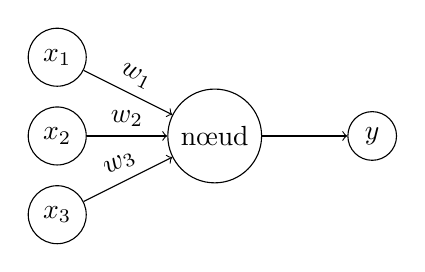
\begin{tikzpicture}
		\node[circle, draw] (n) at (2,2) {n\oe ud};
		\node[circle, draw] (y) at (4, 2) {$y$};
		\foreach \y in {1,2,3} {
			\node[circle, draw] (x-\y) at (0, 4-\y) {$x_\y$};
			\draw[->] (x-\y) -- node[sloped, above, midway] {$w_\y$} (n);
		}
		\draw[->] (n) -> (y);
	\end{tikzpicture}
	\caption{Représentation du réseau de neurone formel}
\end{figure}

Le n\oe ud fait alors une somme pondérée des signaux d'entrée par le poids de leur synapse $\sum_{i=1}^m w_i x_i$ puis utilise une fonction d'activation $\phi$ dont le résultat est envoyé par le signal de sortie $y$.

\begin{equation}
	y = \phi\left(\sum_{i=1}^m w_i x_i \right)
\end{equation}

Dans sa conception, la fonction d'activation permet de reproduire le potentiel d'activation que l'on retrouve dans le domaine de la biologie du cerveau humain. Il s'agit de l'étape qui détermine ou non la transmission de l'information. Grossièrement, il s'agit de dire si oui ou non le neurone s'active.

\paragraph{Fonction d'activation}
Nous pouvons citer les fonctions d'activation les plus répandues : \textit{la fonction seuil}, \textit{la fonction sigmo\"ide}, \textit{la fonction tanh}, \textit{la fonction redresseur}, etc.
\begin{equation}
	\phi_\text{seuil}(x) =
	\begin{cases}
		1 \text{ si } x \geq 0 \\
		0 \text{ si } x < 0
	\end{cases} \qquad
	\phi_\text{redresseur}(x) = \max(x, 0)
\end{equation}
\begin{equation}
	\phi_\text{sigmo\"ide}(x) = \frac{1}{1+\exp(-x)} \qquad
	\phi_\text{tanh}(x) = \frac{1-\exp(-2x)}{1+\exp(-2x)}
\end{equation}

\paragraph{Phase d'apprentissage}
Au cours de son entraînement, nous donnons à notre neurone un vecteur d'entrés $x$ de taille $m$ pour obtenir un résultat $\hat y$.
Nous faisons par la suite une comparaison entre la valeur souhaité $y$ et la valeur obtenue $\hat y$ à l'aide d'une fonction de coût $C$.
Ici l'équation~\ref{eq:cost_function_1} est un exemple de fonction utilisé dans des réseaux de neurones.

\begin{equation}
	\label{eq:cost_function_1} C = \frac{1}{2}(y-\hat y)^2
\end{equation}

L'objectif est de minimiser cette fonction de coût $C$ dont la valeur sert à ajuster les ``poids'' $w$ sur les différents synapses.
\begin{figure}[ht]	
	\centering
	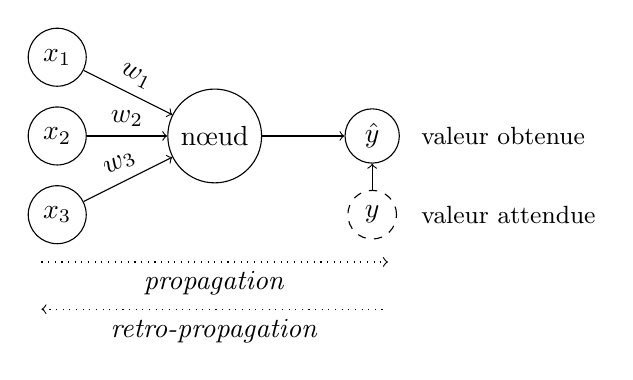
\begin{tikzpicture}
		\node[circle, draw] (n) at (2,2) {n\oe ud};
		\node[circle, draw] (y) at (4, 2) {$\hat y$};
		\node[circle, draw, dashed] (y2) at (4, 1) {$y$};
		\node[right=.5cm] at (y) {\small valeur obtenue};
		\node[right=.5cm] at (y2) {\small valeur attendue};
		\draw[->] (y2) -- (y);

		\foreach \y in {1,2,3} {
			\node[circle, draw] (x-\y) at (0, 4-\y) {$x_\y$};
			\draw[->] (x-\y) -- node[sloped, above, midway] {$w_\y$} (n);
		}
		\draw[->] (n) -> (y);

		\draw[->, dotted] (-.2, .4) -- node[midway, below] {\textit{propagation}} (4.2, .4);
		\draw[<-, dotted] (-.2, -.2) -- node[midway, below] {\textit{retro-propagation}} (4.2, -.2);
	\end{tikzpicture}
	\caption{Représentation du réseau de neurone formel}
\end{figure}
Lorsque les données parcourent le réseau de neurones de gauche à droite on parle alors de \textit{propagation}.
Tandis que lors de l'ajustement des poids, les données remontent le réseau de neurones de droite à gauche et nous parlons alors de \textit{retro-propagation}.

\paragraph{Fonction Co\^ut}

Comme nous venons de le voir, le fonction co\^ut joue un r\^ole important lors de l'apprentissage du neurone.
Il en existe plusieurs, chacunes ayant des avantages et inconvénients, certaines sont orientés sur des calculs de distribution tandis que d'autres sont plus efficaces sur des calculs de zones. Nous allons aborder certaines fonctions de manière non-exhaustives :

\subparagraph{Binary Cross-Entropy} Cette fonction mesure la différence entre deux probabilité de distribution pour une variable prise aléatoirement.

\begin{equation}
	C_p (q) = - \frac{1}{N} \sum_{i=1}^{N} y_i \log(p(y_i)) + (1 - y_i)\log(1-p(y_i))
\end{equation}

\subparagraph{Categorical Cross-Entropy}

\begin{equation}
	C = - \sum_{i = 1}^{C} t_i \log(f(s)_i)
\end{equation}

\subparagraph{Weighted Cross-Entropy}

\subparagraph{Soft Dice}

\subparagraph{Pixel-Wise Cross-Entropy}

\subparagraph{Lovasz Hinge}

\paragraph{Algorithme du gradient}
Calcul de la dérivé d'une fonction pour en trouver un résultat optimal

\subparagraph{Algorithme du gradient stochastique}
Au lieu de reévaluer les poids pour un epoch donné, l'algorithme du gradient stochastique va les modifier dès la première évaluation et ainsi de suite.

\subsection{Conception d'un réseau de neurones}
Dans cette partie, nous allons mettre en \oe uvre un \gls{ANN} à l'aide de python.


	\section{Convolutionnal Neural Network}
\gls{CNN}

\subsection{Feature extraction}

\subsection{CBIR: Content Based Image Retrieval}


	\section{Recurent Neural Network}

\gls{RNN}
Réseau de neurones avec une boucle temporelle.
La couche cachée produit une sortie à la fois vers le dernier niveau mais renvoit également sa sortie dans son entrée.

\begin{figure}[ht]
	\centering
	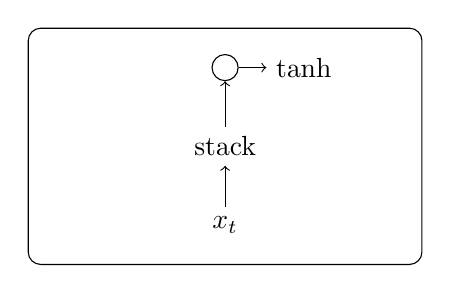
\begin{tikzpicture}
		\draw[rounded corners=4.5pt] (0, 0) rectangle (5, 3);

		\node[circle, draw] (node) at (2.5, 2.5) {};
		\node (stackfunc) at (2.5, 1.5) {stack};
		\node (outputfunc) at (3.5, 2.5) {tanh};
		\node (entry) at (2.5, .5) {$x_t$};

		\draw[->] (node) -- (outputfunc);
		\draw[->] (stackfunc) -- (node);
		\draw[->] (entry) -- (stackfunc);
	\end{tikzpicture}
	\caption{Représentation simplifiée d'un réseau de neurones récurrent}
\end{figure}

\paragraph{One to Many}

\paragraph{Many to One}

\subsection{\gls{LSTM}}

\paragraph{forget gate}
\begin{equation}
	f_t = \sigma(W_f [h_{t-1}, x_t] + b_f)
\end{equation}

	\part{Unsupervised learning}

	À la différence de l'apprentissage supervisé, nos données ne disposent pas de labels.
	Impossible donc d'entraîner un algorithme en fonction d'une valeur attendue, cette solution permet cependant d'identifier des motifs dans notre jeu de données.

	\paragraph{Application d'apprentissage non-supervisé}
	Parmis les applications d'apprentissage non-supervisé, nous allons dénoter une utilisation plus fréquente dans le cadre de la détection d'anomalies et la segmentation en groupe.

	\subparagraph{Anomaly Detection} Les système de détections d'anomalies sont utilisé pour repérer des fraudes ou des évènements qui dénotent d'une certaine tendance.

	\subparagraph{Group segmentation}
	Les algorithmes de segmentation sont utilisé pour classifier du contenu, des données en fonction de leurs similarités.

	\chapter{Réduction de dimensions}
	\section{Projection linéaire}
	\section{Manifold Learning}


	\chapter{Clustering}
	Utiliser un algorithme de \textit{clustering} vise à identifier différentes classes d'un jeu de données.
	Pour ce faire, on identifie plusieurs sous-ensembles que l'on groupe en fonction de leurs similarités.

	\section{K-means}


	\section{DBSCAN}
	\textsc{dbscan} utilise un paramètre \textit{min\_samples} pour identifier les sous-ensembles de taille suffisante.
	Si deux sous-ensembles sont à proximité, celui dont la densité est la plus grande l'emporte sur le second.

	\inputminted{python}{code/machine-learning/unsupervised-learning/dbscan.py}

	\chapter{Feature Extraction}

	\section{Autoencoders}

	\chapter{Self Organizing Map}

L'objectif premier d'une SOM est de réduire la dimension du vecteur d'entré. L'algorithme cherche à réaliser une carte suffisamment représentative des charatéristiques en perdant le moins d'informations possible.



\end{document}
